\section{Cámara}
Para animar el movimiento de la cámara he utilizado un \textit{Dummy} y he puesto como hijo a la propia cámara sin su \textit{Target}. Asimismo, he puesto el \textit{Target} de la cámara para que apunte al centro de la escena. Con esto, ya es posible animar el giro de la cámara sin demasiada complicación y permitiendo que siempre esté apuntando hacia la escena.

\bigskip

Los \textit{keyframes} de la cámara son:

\begin{itemize}
   \item \textbf{Instante 0: }La cámara se encuentra en la posición inicial, con una perspectiva similar a la que aparece en el guion.
   \item \textbf{Instante 150: }La cámara se encuentra en su posición final, que en este caso he decidido que sea la misma, para que haga una rotación completa en los 5 segundos.
\end{itemize}

\bigskip

La curva de animación del \textit{Dummy} de la cámara es:

\begin{figure}[H]
   \centering
   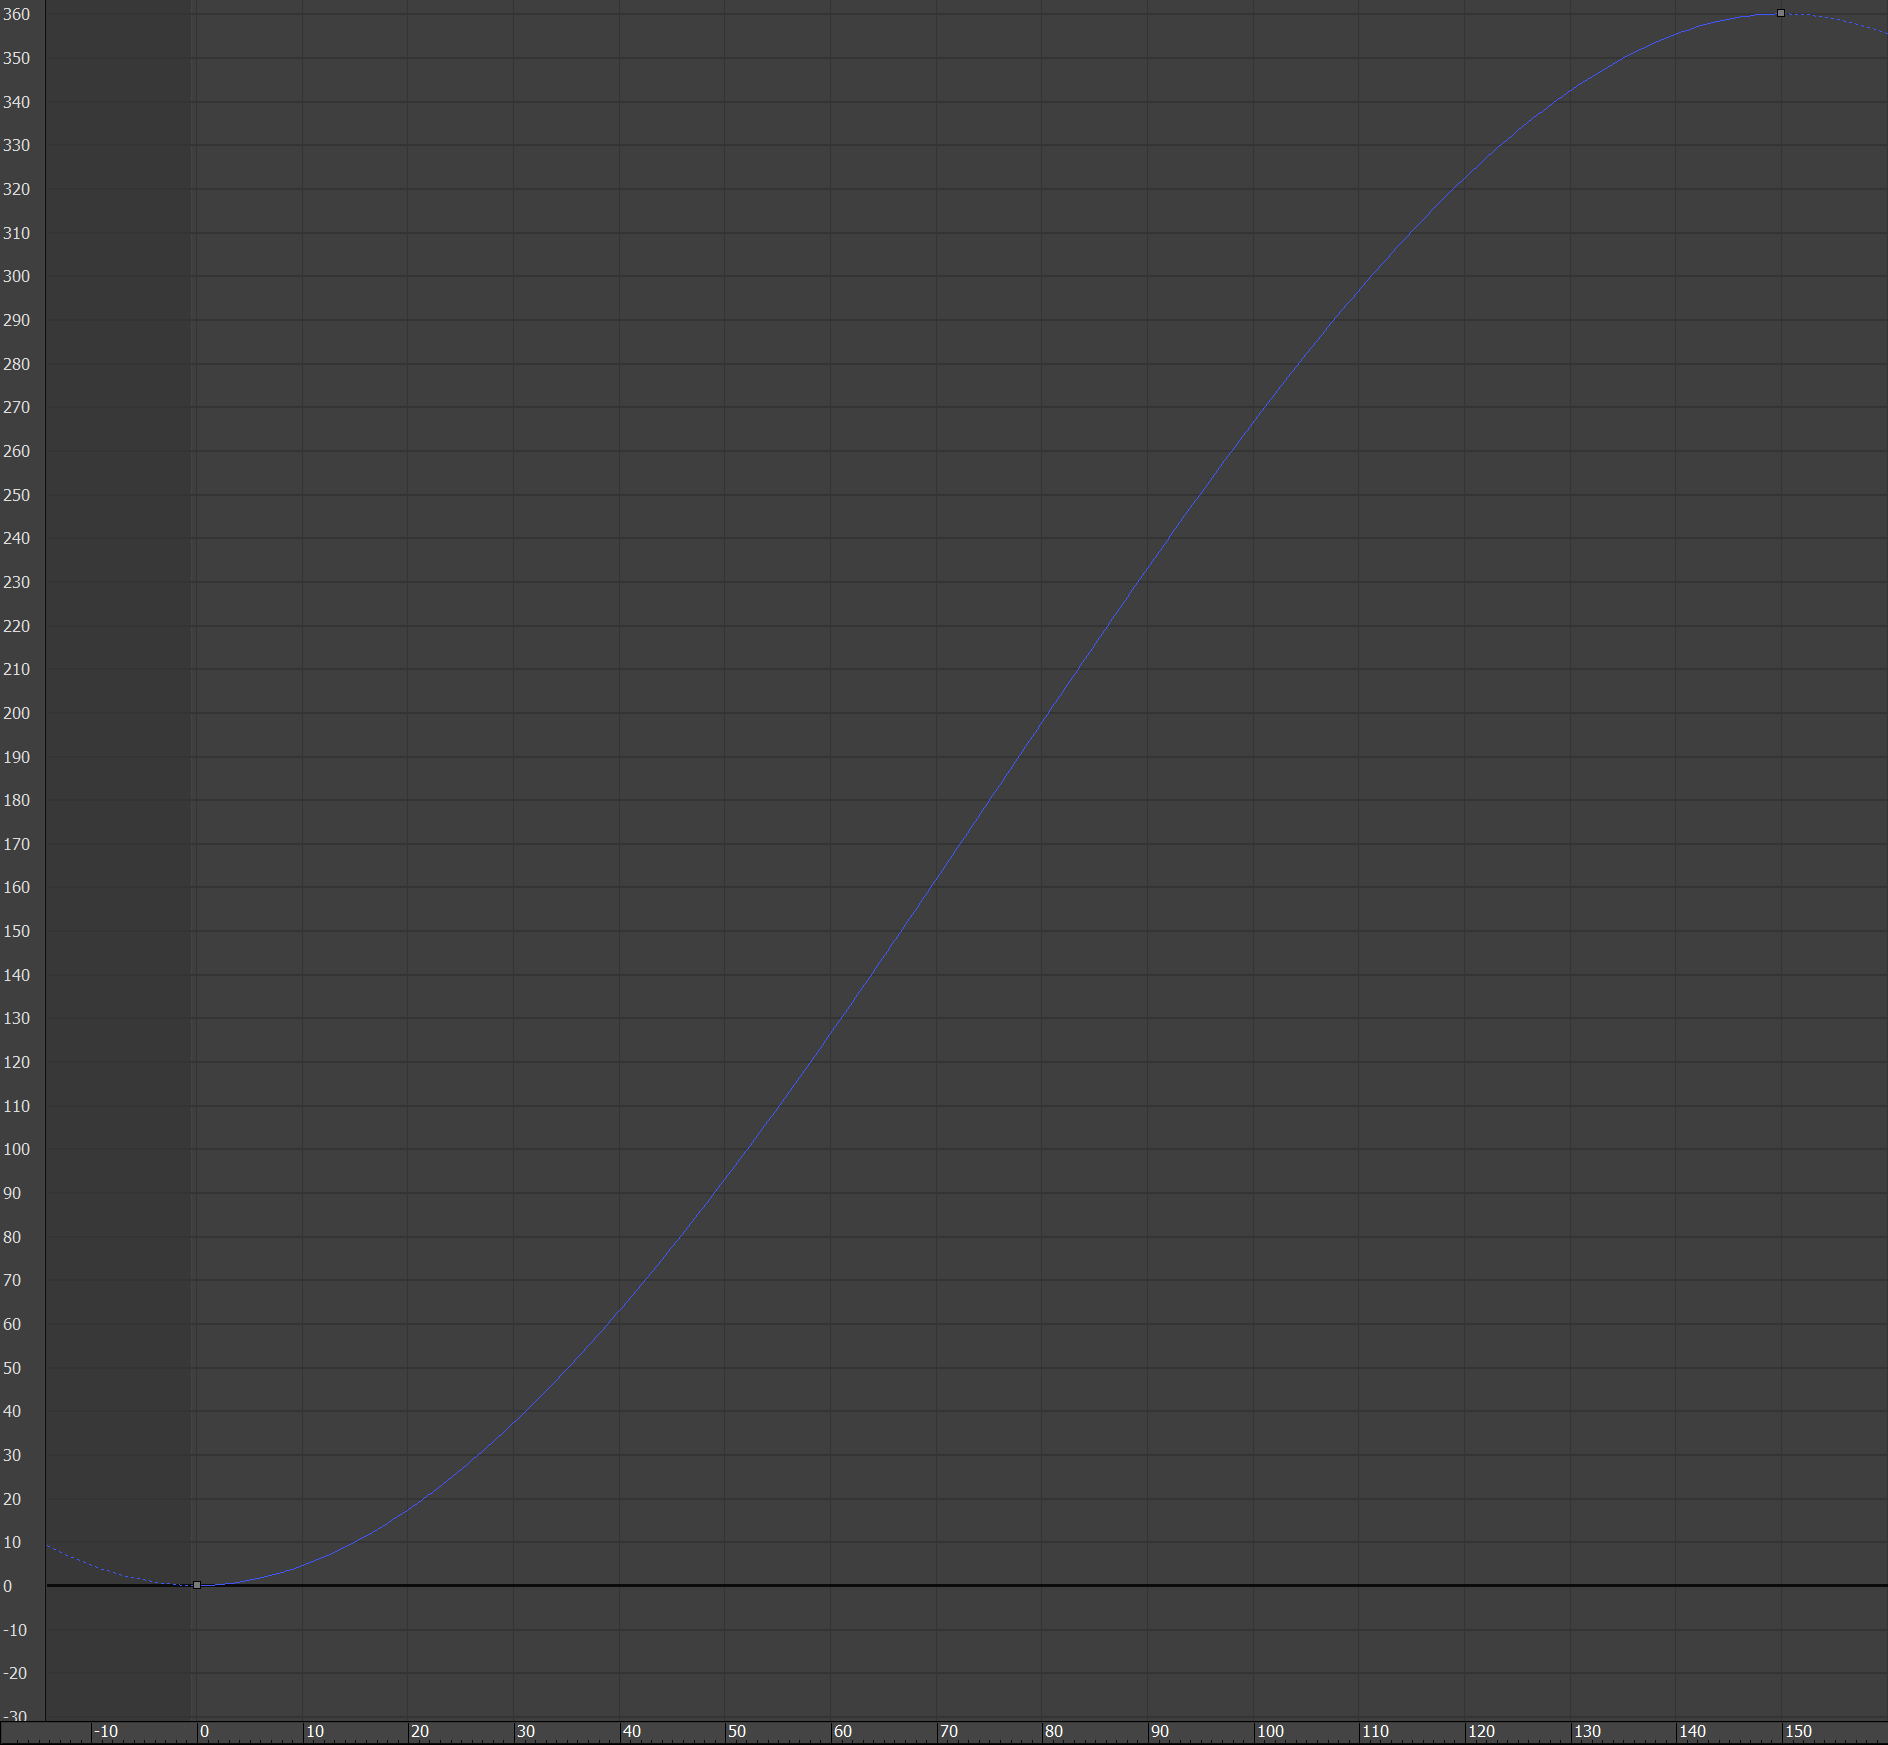
\includegraphics[width=0.6\textwidth]{imagenes/curvas/Camara/blue.png}
   \caption{Curva que representa la rotación en el eje Z con respecto al tiempo.}
\end{figure}

Como se puede observar, he utilizado una función \textit{Slow-in/Slow-out}, para dar una sensación más realista al hacer la animación inversa, ya que de la otra forma parecía demasiado robótico.

\newpage

La trayectoria que sigue es la siguiente:

\begin{figure}[H]
   \centering
   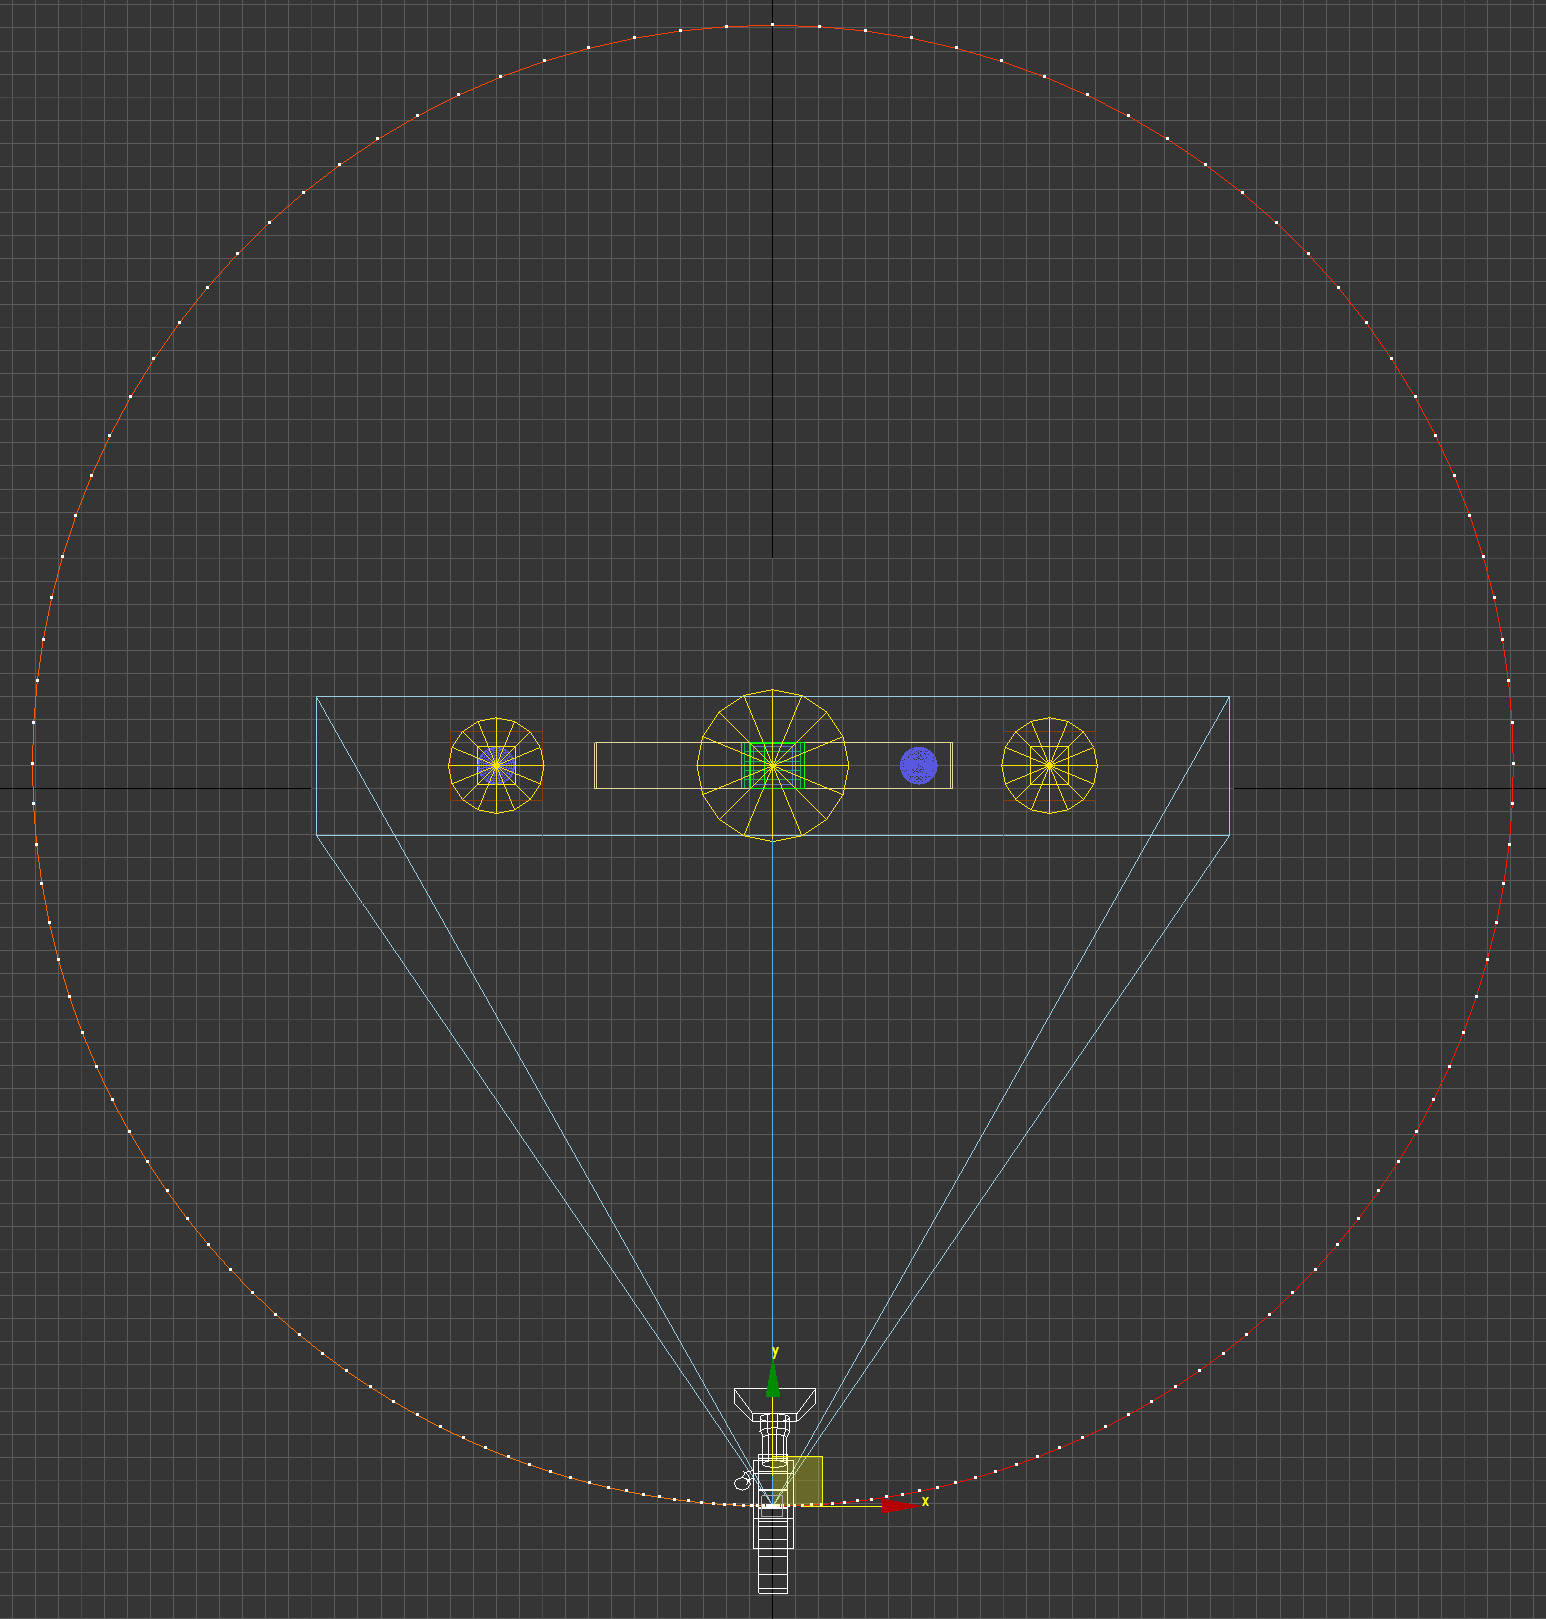
\includegraphics[width=0.5\textwidth]{imagenes/misc/CameraPath.png}
   \caption{Trayectoria final seguida por la cámara.}
\end{figure}

\bigskip

Y la posición del \textit{Dummy} y la cámara para que funcione correctamente es:

\begin{figure}[H]
   \centering
   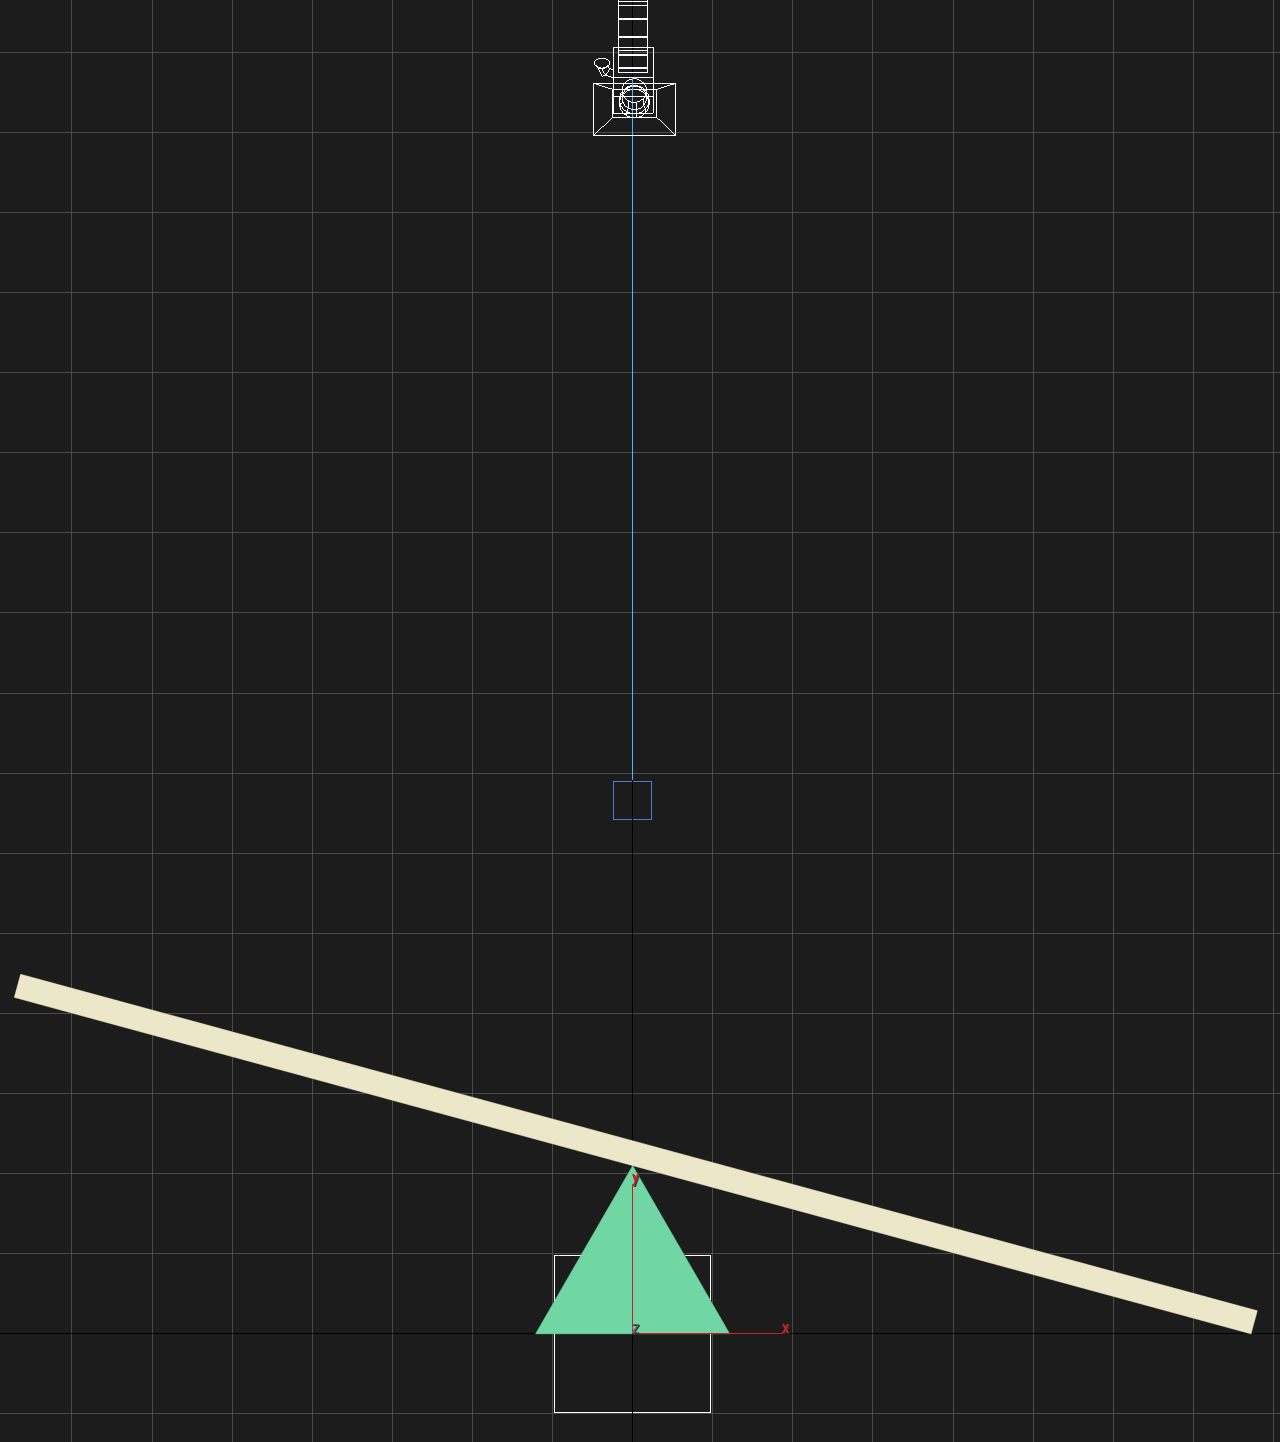
\includegraphics[width=0.5\textwidth]{imagenes/misc/DummyCamera.png}
   \caption{Cámara junto a su \textit{Dummy} en la escena. Así se consigue que la cámara apunte siempre a los objetos.}
\end{figure}

\newpage